\chapter{Luminosity  Measurement and Calibration}
\label{ch3}
%%%%%%%%%%%%%%Introduction%%%%%%%%%%%%%%%%%%%%

The precision measurement of the luminosity delivered to the CMS by the LHC is important for a variety of reasons. Online, the luminosity measurement provides realtime feedback on the LHC performance and operation. Offline, the luminosity measurement is a crucial component of physics analysis, either for measuring the cross section of observed processes or for setting upper limits in searches for processes BSM \cite{pas_18}.\\
A total of seven systems are used for measuring luminosity at CMS. These systems are referred to as luminometers.  Each luminometer reads out a rate of the specific quantities observed in the detector (hits, tracks, clusters, etc.). This rate, R, should be proportional to the instantaneous luminosity,$\mathcal{L}_{inst}$, with the constant of proportionality given by the visible cross section $\sigma_{vis}$ \cite{pas_18}:

\begin{equation}
R=\mathcal{L}_{inst}\sigma_{vis}
\label{lumi_exp_gen}
\end{equation}

The determination of $\sigma_{vis}$ is carried out through van der Meer (vdM) scans performed with a dedicated LHC machine setup, exploited by S. Van der Meer for luminosity measurements at ISR \cite{vdM_cal}.

\section{Pixel Cluster Counting method}
The Pixel Cluster Counting method exploits the very large number of pixels in the tracker of the CMS detector. At design luminosity of $10^{34}cm^{-2}s^{-1}$, the detector occupancy is less than 0.1\% on average (the average number of clusters per minimum bias interaction is about 50 and the average number of pixels per cluster is about 5) \cite{pas-13}. The very low occupancy leads to an excellent linear detector response with increasing LHC luminosity \cite{pas_18}. \\
The PCC method uses the rate of pixel clusters in the CMS pixel detector to provide an offline luminosity measurement. Pixel clusters are formed from adjacent pixels, as mentioned in section \ref{pixel_clust_reco}. PCC measurement uses the data collected with the standard CMS trigger system with triggers requiring colliding bunches but not any specific event activity; this is referred as "zero-bias trigger'' \cite{pas_18}.\\
Each bunch crossing gives rise to some number of pp interactions, with each such interaction resulting in some number of pixel clusters. If the average over several zero-bias events is taken, the mean number of pixel clusters per event is \cite{PCC_PAS_12_001}:

\begin{equation}
\left < N_{\text{cluster}} \right > = \left < N_{\text{pixel}/\text{interaction}} \right >  \left < N_{\text{interactions}} \right > \equiv \left < N_{\text{pixel}/\text{interaction}} \right > \mu
\end{equation}

where in the last step, the average number of interactions per bunch crossing, pileup, is denoted by the symbol $\mu$.

%%%%%%%%%%%%%%%%%%%%%%%%%%%%%%%%%%%%%%%%%%%%%%%%%%%%%%%%%%%%%%%%%%%%%%%%%%%%%%%%%%%%%%%%%

\section{Luminosity calibration: van der Meer method}
In the practice, as mentioned in chapter 1, the properties of the colliding beams are not know precisely, such as the bunch density profile, so that the integral in \ref{lumi_2} cannot be solved analytically. In LHC a experimental techinque know as vdM method is implemented  with a dedicated machine setup to bring the bunch density profiles close to Guassian distributions.\\
The VdM scan method, %, exploited by S. Van der Meer for luminosity measurements at ISR  \cite{vdM_cal} and
applied by LHC Experiments in Run 1 and Run 2, allows to measure and evaluate the integral over the proton bunch densities in eq. \ref{lumi_2}. For the vdM scan method to be applicable it is also assumed that the two bunch $\rho$ can be factorized into independent terms in x and y \cite{pas-15}.  The value of the two beam overlap integrals in Eq. (2) is determined by varying the beam separation and measuring the resulting rates \cite{pas_18}:

\begin{equation}
\int \rho_{x1}(x) \rho_{x2}(x) dx = \frac{R_{x}(0)}{\int R_{x}(\Delta) d\Delta}
\end{equation}

where $R_{x}(\Delta)$ is the rate measured when the two beams are separated in x by a distance $\Delta$; a asimilar equation can be written in y. Then the beam overlap width $\Sigma_{x}$ (and similarly $\Sigma_{y}$) is defined as \cite{pas_18}:

\begin{equation}
\Sigma_{x}= \frac{1}{\sqrt{2\pi}} \frac{\int R_{x}(\Delta)d\Delta}{R_{x}(0)}
\end{equation}

yielding the final expression for luminosity (for one single bunch):

\begin{equation}
\mathcal{L}_{inst}=\frac{N_{1} N_{2}f}{2 \pi \Sigma_{x}\Sigma_{y}}
\end{equation}

where $N_{1,2}$ are the particles per bunch (bunch current) and  $f= 11246$ Hz is the bunch orbit frequency around the LHC ring.\\
This expression can be finally used in \ref{lumi_exp_gen} to get $\sigma_{vis}$:

\begin{equation}
  \sigma_{vis}=\frac{2\pi \Sigma_{x} \Sigma_{y} R(0, 0)}{N_{1}N_{2} f}
  \label{sigmavis_eq}
\end{equation}

Experimentally, two separate scans in the x and y directions are performed. The beams are scanned against each other  while measuring the rate (normalized by the product of the beam currents) at a certain number of separation steps, fitting the resulting points with a functional form, and using the fitted function to extract $\Sigma_{x,y}$ and $R(0,0)$ in \ref{sigmavis_eq}. Fig. \ref{vdm_sketch} shows an sketch of the beam positions during vdM scans in X and Y planes together with the detector rate as a function of beam separation.

\begin{center}
  \begin{figure}[ht]
    \centering
    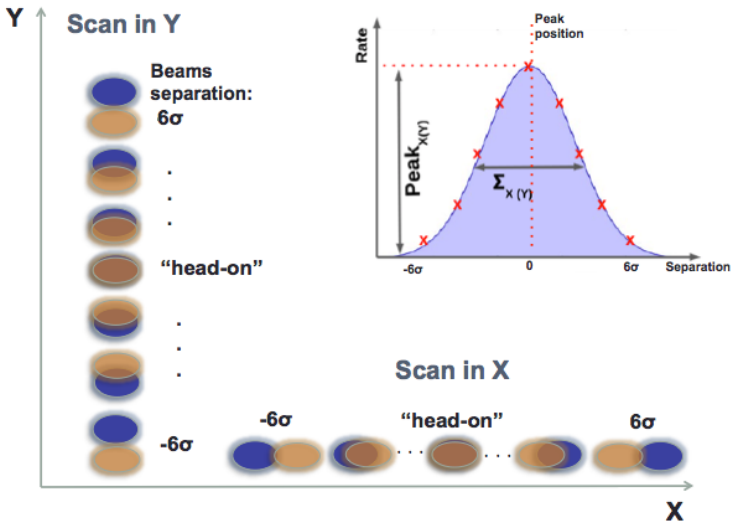
\includegraphics[scale=.37]{Chapter3/vdm_sketch.png}
    \caption[Sketch of a vdM scan in X and Y planes and example of fitting resulting rates]{ The sketch of a vdM scan in X and Y planes. The indent sketch is an example of the fitting of the resulting rates \cite{vdM_sketch}.}
    \label{vdm_sketch}
  \end{figure}
\end{center}

%In practice, the integral in Eq. (4) is evaluated by performing two separate scans in the x and y directions, measuring the rate (normalized by the product of the beam currents) at a certain number of separation steps, fitting the resulting points with a functional form, and using the fitted function to determine the overall integral [PAS-18]. ADD HEDWING FIGURE. "this is illsutrated in fig N". Once Σx and Σy are determined, then Eq. (1) can be used to obtain the overall visible cross section σvis [pas-18].

%NOTA: Hay un pas, creo,en donde dicen lode beam current normalizado, haciendo referencia a la gráfica. Pero tal vez esto vendría en la siguiente seeción, la de resultados, ya que muestre las fitted graphs.


% https://pos.sissa.it/364/194/pdf



%DUDA: En la qe. lumi_2 decimos n_b colliding bunches y aquí hablaremos de solo un coliding buch. Lumi inst. se refiere a un solo coliding bunch? Cuál es la diferencia? En el vdM Scan usamos un solo colliding bunch?

\subsection*{Backgrounds}
Before performing the fit to extract $\Sigma_{x}$ and $\Sigma_{y}$, the raw measured rates must be corrected for background in the detector. The background contribution is estimated independently, using a special period known as Super Separation period where the beams are separated, ensuring that the only contribution is from background either beam-induced background or detector noise. There are three sources of beam-induced background: Beam Gas Elastic (BGE), Beam Gas Inelastic (BGI) and Beam Halo (BH). BGE contribution are all coherent and quasi-elastic nuclear elastic and coulomb scattering for multi-turn beam-gas interactions around the ring; typically the interaction of the primary beam proton and the aperture takes place at the collimator. BGI  are all inelastic interactions of primary beam protons with rest gas in the beam pipe. The interaction rate is dominated by the vacuum quality in the various beam line elements upstream CMS; therefore the origin of this contribution is distributed all along the long straight section. BH component is caused by the inefficiency of the main collimation system. Protons can escape from one collimator and being intercepted by another collimator \cite{bkg_source}.\\
%https://cds.cern.ch/record/1316945/files/CR2010_169.pdf
%https://cds.cern.ch/record/2816679/files/document.pdf
% Electronic noise?:
%  https://cds.cern.ch/record/1293521/files/Thesis-2002-Gu.pdf
Several other corrections are applied to the raw data before the vdM fit is performed.\\
%These corrections take into account drifts in the position of the LHC orbit, beam-beam interaction effects, and the beam separation length scale. The intensities are measured by the LHC beam current monitors and are corrected for bunched spurious (so-called “ghost” and “satellite”) charges \cite{pas_18}.

%----------- MOVE TO NEXT CHAPTER-------------%

%Before performing the fit to extract $\Sigma_{x}$ and $\Sigma_{y}$, the raw measured rates must be corrected for background in the detector. The background contribution is estimated independently, using two special periods, each 5 minutes long, during the VdM scan where the beams were separated by 6$\sigma$ (where $\sigma_{b}$ is the beam size) in both $x$ and $y$ directions, ensuring that the only contribution is from background (either beam-induced background or detector noise). The estimated background is then subtracted from the raw data before the fit is performed using a Gaussian-kind  function, which was found in 2018 to adequately describe the measured rates as a function of beam separation.\\
%Several other corrections are applied to the raw data before the VdM fit is performed. These corrections take into account drifts in the position of the LHC%orbit, beam-beam interaction effects, and the beam separation length scale. The event rates are normalized by the bunch intensities before the fit. The intensities are measured by the LHC beam current monitors and are corrected for bunched spurious (so-called “ghost” and “satellite”) charges.



%\section{Data set: 2018 vdm scan program}
%
%For 2018, the VdM scans were performed during LHC fill 6868 on June 30 and July 1 at $\sqrt{s}=13 \text{TeV}$. The LHC filling scheme used  124 colliding bunch pairs at the CMS interaction point (IP5) widely spread over the orbit to reduce long-range beam-beam effects and detector afterglow.  The resulting beam size $\sigma_{b}$ at the beginning of the fill was in the range of approximately 85–95 and 80–90 $\mu$m in x and y, respectively, increasing over time in the x dimension and decreasing over time in the y dimension. No crossing angle was used for collisions. The resulting peak pileup was approximately $\mu$ = 0.6, much lower than in a regular physics fill \cite{pas_18}.\\
%The bunch intensities were approximately 7–9$\times 10^{10}$ protons per filled bunch, resulting in a total beam intensity of slightly above $10^{10}$ protons per beam. The total beam intensities were measured with the DC Current Transformers (DCCT), and the bunch currents were measured with the Fast Beam Current Transformers (FBCT) \cite{pas_18}.\\
%To ensure a dataset with a high event count for PCC even at large beam separations, CMS gated the zero-bias triggers on 5 bunch pairs (BCIDs 265, 865, 1780, 2192, and 3380) and recorded events with a total rate of 27.7 kHz \cite{pas_18}.\\
%The CMS VdM scan program was conducted in two parts (``takes'') due to an alarm. Apart from the vdM scans other studies were carried out. Betwen that studies, only the imaging scans are used to compute $\sigma_{vis}$. The standar vdM scans are referred as ``norm'' and the imaging scans as ``img''. In the first take of the VdM scan program a vdM scan ``norm1'' and a imaging scan ``img1'' were carried out. The second part consisted of the scans ``img2'', ``img3'', ``norm2'', ``norm3'' and ``norm4'' were done. In total are 7 scans to determine $\sigma_{vis}$ \cite{pas_18}.\\
%In the vdM scans the two beams were separated by $6 \sigma_{b} \approx 600 \mu$m and scanned across one another in a sequence of 25 steps with 30 seconds per step. For the beam imaging scans  one beam (beam 1 in the first pair, followed by beam 2 in the second pair) is kept fixed at its nominal position while the other is separated and scanned in 19 steps from  $+$4.5$\sigma_{b}$ to $-$4.5$\sigma_{b}$ with 46 seconds per step. In each of both scans (scan  pairs), the scan was performed first in the x direction and then in the y direction \cite{pas_18}.\\
%Fig. \ref{scan_prog}  shows the beam positions for the two beams in the x and y directions as measured by the DOROS BPMs during the scan program, showing all scan pairs of the 2018 scan program.
%
%\begin{center}
%  \begin{figure}[ht]
%    \centering
%    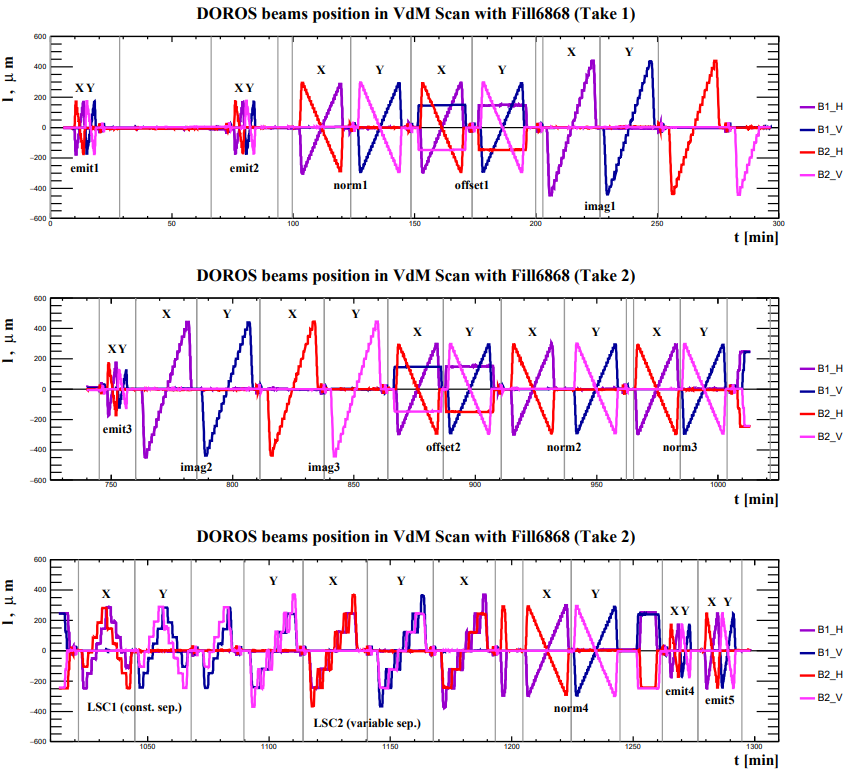
\includegraphics[scale=.45]{Chapter4/2018Scanprogram.png}
%    \caption[2018 scan program]{Relative change in beam positions measured by the DOROS BPMs during the 2018 scan program for the two individual beams in the horizontal x and vertical y planes, as a function of the elapsed time from the beginning of the program. The top row shows the take 1 of the program before the alarm at CMS, while the bottom two rows show the program after the alarm \cite{pas_18}.}
%    \label{scan_prog}
%  \end{figure}
%\end{center}
%
%


%%%%%%%%%%%%%%%%%%%%%%%%%%%%%%%%%%%%%%%%%%%%%%%%%%%%%%%%%%%%%%%%%%%%%%%%%%%%%%%%%%%%%%%%%%%%%%%%%%%%%%%%%%%%%%%%%%%

